\documentclass{article}
\usepackage[utf8]{inputenc}
\usepackage{amsmath}
\usepackage{graphicx}
\usepackage{pdfpages}

\begin{document}
\section{Probability Theory Review}
\subsection{Probabilistic Independence}
\begin{itemize}
	\item[a)]
	With rolling the dice twice you have 36 different outcomes. Event A gets fullfilled in 3 cases. 12 cases fullfil event B and C. Event D gets fullfilled in 15 cases. And 22 cases for Event E.
	This results in following Propabilties for the different events:
	$$P(A) = \frac{3}{36}=\frac{1}{12}$$$$P(B) =\frac{12}{36}=\frac{1}{3}$$$$ P(C) = \frac{12}{36}=\frac{1}{3}$$$$P(D) = \frac{15}{36}=\frac{5}{12}$$$$P(E) = \frac{22}{36}=\frac{11}{18}$$ 
	\item[b)] Event A and B get satisfied in the cases (6,5),(5,6),(6,6) to show dependece we have to show following equation.
	$$P(A \cap B) \neq P(A)P(B)$$
	$$P(A \cap B)=\frac{3}{36} \neq \frac{1}{36} = \frac{3}{36}*\frac{1}{3} = P(A) * P(B)$$
	since both sites are not equal we know that A is dependent of event B.
	\item[c)]
	$A\cap C$ can not be fullfilled. And since $P(A)>0$ and $P(C)>0$ we know that
	$$P(A\cap C) = 0 \neq P(A)P(C)>0$$
	Which shows that A is depented of event C.
	\item[d)]
	$D\cap E$ gets satisfied by the cases (1,2),(2,3),(3,4),(4,5),(5,6) which implies $P(D\cap E)=\frac{5}{36}$
	Since $$P(D\cap E) = \frac{5}{36} \neq \frac{55}{216}=\frac{5}{12}*\frac{11}{18} = P(D)P(E)$$ we know that D and E are dependend.
\end{itemize}
\subsection{Communication through a Noisy Channel}
\begin{itemize}
	\item[a)]
	For a random variable of source X, the probability mass function can be denoted as:
	
	$$P_X(x_k)=\ P(X=x_k), \ for\: k={0,1}$$
    So for the source symbol 0 
    $$ P_X(0)=P(X=0)=p$$
    and for 1 
    $$ P_X(1)=P(X=1)=1-p$$
    \item[b)]
	Y is the random variable of the receiver symbol which can have the value 0 and 1. So the mass function of Y given X which implies the channel's error probability  is as follows:
	
	$$P_Y(y_k)=\ P(Y=y_k), \ for\: k={0,1}$$
	
    $$P_Y(0 \: | \:(X=x_k=1))= \epsilon_1$$
    $$P_Y(1 \: | \:(X=x_k=0))= \epsilon_0$$

    \item[c)]
    The probability of transmitting the symbol sequence "1001110" is:
    $$(1-p)^4 . p^3$$
	\item[d)]
	Let, c denotes receiving the signal correctly. The probability of randomly chosen symbol which is received correctly is:
	$$ P(c) = P(c \: | \: 0 ).P(0)+ P(c \: |\:   1).P(1)$$
	$$=p.(1-\epsilon_0)+(1-p).(1-\epsilon_1)$$
	
	\item[e)]
	The probability of receiving the transmitted symbol sequence 1011 correctly is:
	$$ P(C) = P(1\:\: C)^3.P(0\:\: C), where\:C\:=\:receiving \: correctly$$ 
	$$=(1-\epsilon_1)^3.(1-\epsilon_0)$$
	\item[f)]
	The probability of receiving "1101" is as follows: [R=Receiving, T=Transmitting]
	$$P(R\:1101)=(P(R1\:|\:T1).P(T1)+$$ 
	$$P(R1\: |\: T0).P(T0))^3 . P(R0\: | \:T1).P(T1)+
	P(R0\: |\: T0).P(T0))$$
	$$=((1-\epsilon_1).(1-p)+\epsilon_0.p)^3.(\epsilon_0.(1-p)+(1-\epsilon_0).p)$$
	\item[g)]
	Probability of receiving a transmitted O[000] correctly after introducing redundancy:
	$$P(000,001,010,100\:|\:000)$$
	$$=P(000\:|\:000)+P(001\:|\:000)+P(010\:|\:000)+P(100\:|\:000)$$
	$$=(1-\epsilon_0)^3+3.(1-\epsilon_0)^2.\epsilon_0$$
   \item[h)] 
    The probability of transmitting 0[000] that the received signal is 101:
    $$P(000\:|\:101)=\frac{P(000\land101)}{P(101)}$$
    $$=\frac{P(101\:|\:000).P(000)}{P(101\:|\:000).P(000)+P(101\:|\:111).P(111)}$$
    $$ \frac{\epsilon_0^2(1-\epsilon_0).p}{\epsilon_0^2(1-\epsilon_0).p+(1-\epsilon_1)^2.\epsilon_1.(1-p)} $$
	\item[i)]
	The noisy channel can be a good model of human communication with natural languages. It actually removes the part of guessing by getting close to the optimal channel capacity. Evaluating the results of the design assists to develop the system even more. By applying some variants like the question g, it can be designed such a way that the optimal performance is more achievable. It has its impact on Handwriting recognition, Text Generation, Machine Translation and so on.   
\end{itemize}
\section{Character N-grams and Entropy}
\subsection{N-grams Frequency Analysis}
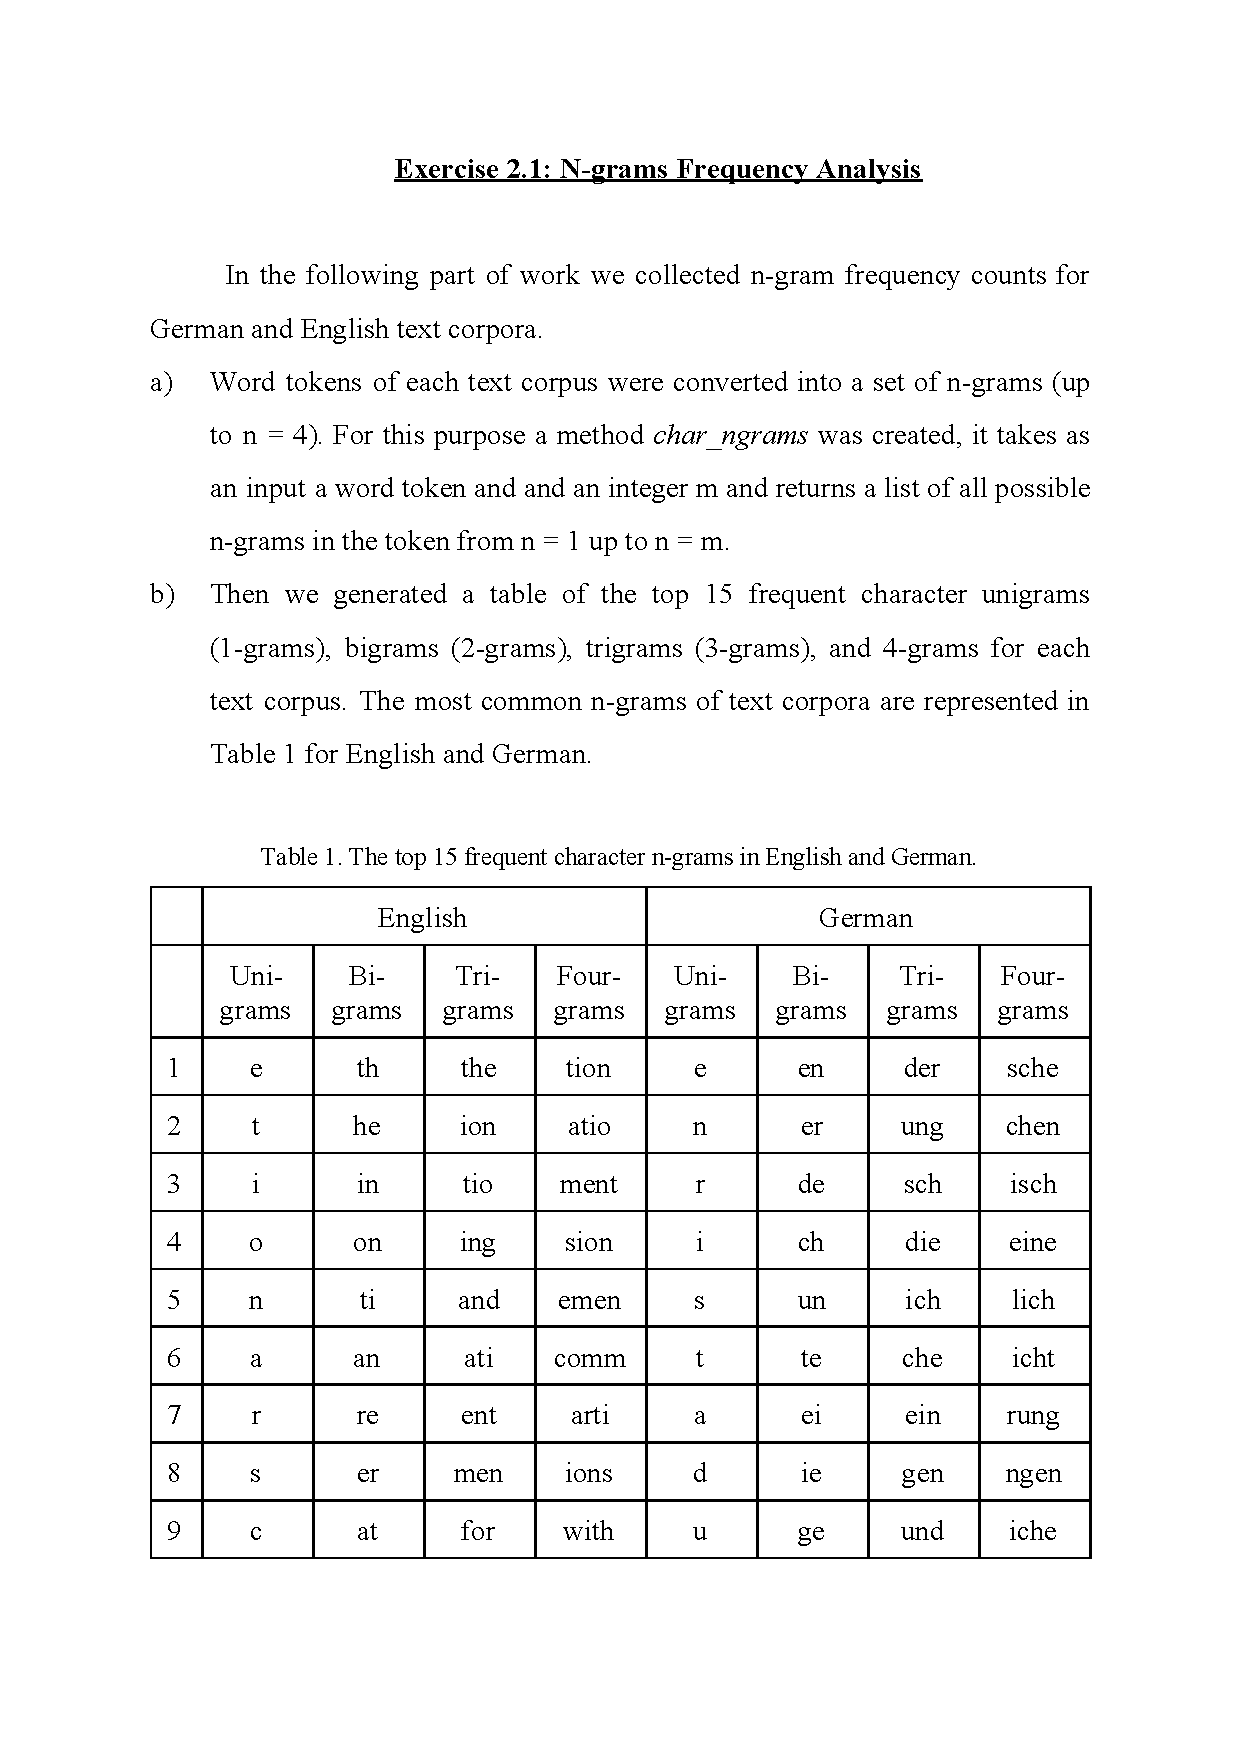
\includepdf[pages=-]{Ex21.pdf}
\subsection{N-gram Probability Distributions}
\begin{itemize}
	\item[a)]
	see prob\_dist.py
    We gave out the probability for an empty history if for the given historie no possible following character was found in the n-grams to ensure that the sum of the probability distribution always sums up to one. This was tested with assert and different histories.
    \item[b)]Below are the plots for the probability distribution for the histories `', `n', `un' and `gun'. We can observe that with a growing history we get less and less possible characters based on the n-grams collected on the sample. In the first case with an empty history, every character is possible even if some are more probable than others. With `n' as history, some of the characters get eliminated. With the biggest history `gun' we can see that there are only two possible characters that can follow: g and s, where g has a high probability since it was more frequent in the sample.
    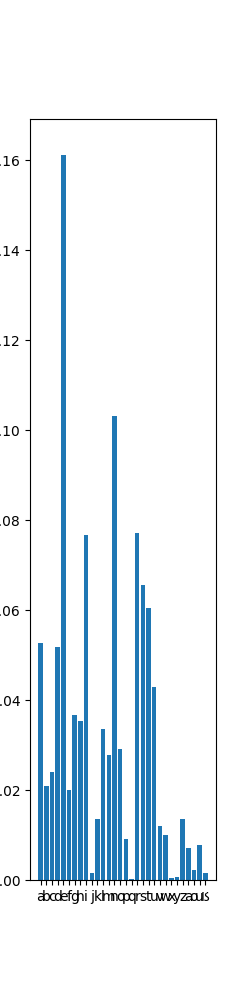
\includegraphics[width=\textwidth]{./plots/emptyhistory.png}
	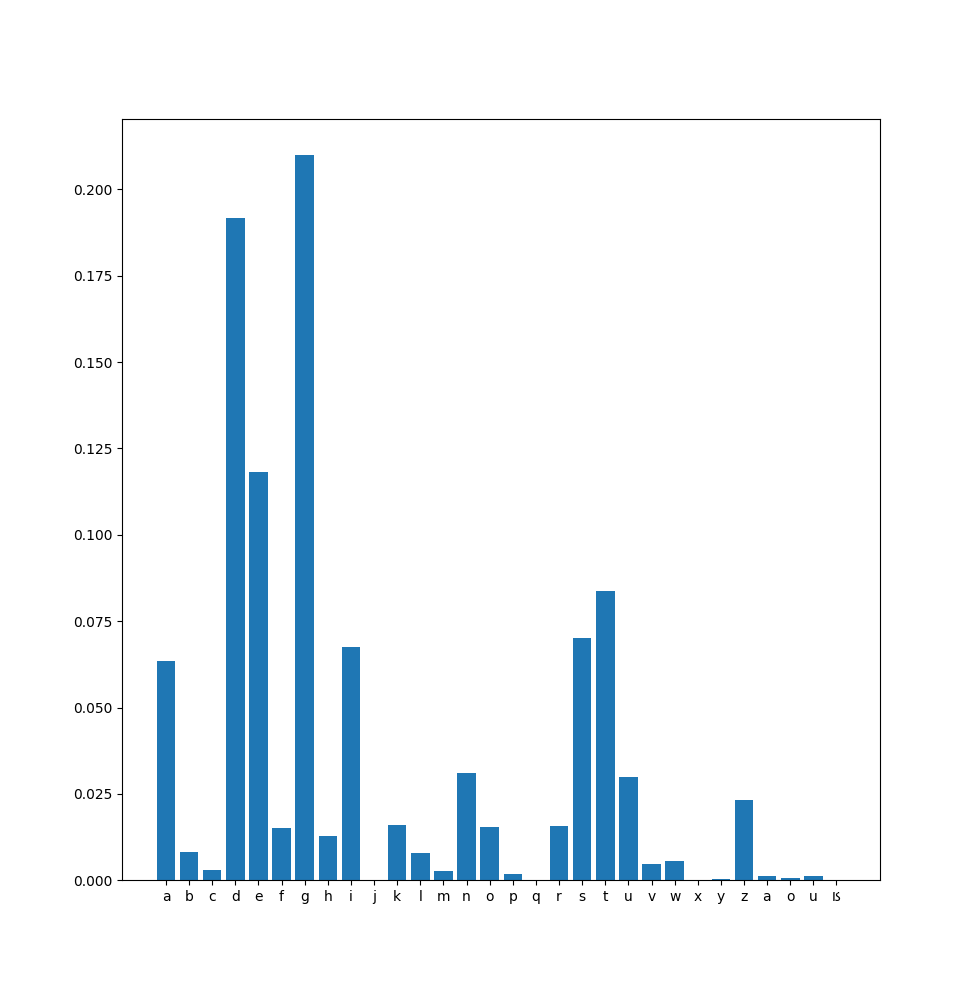
\includegraphics[width=\textwidth]{./plots/nhistory.png}
	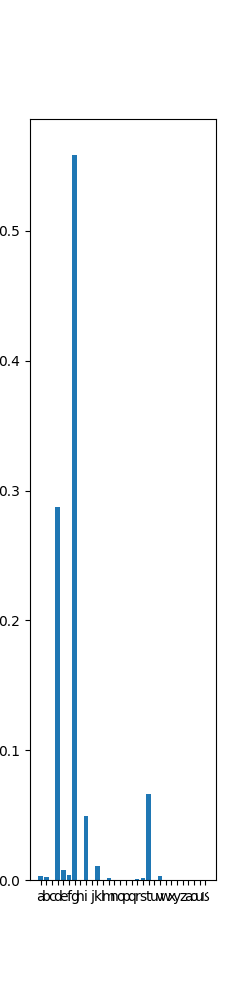
\includegraphics[width=\textwidth]{./plots/unhistory.png}
	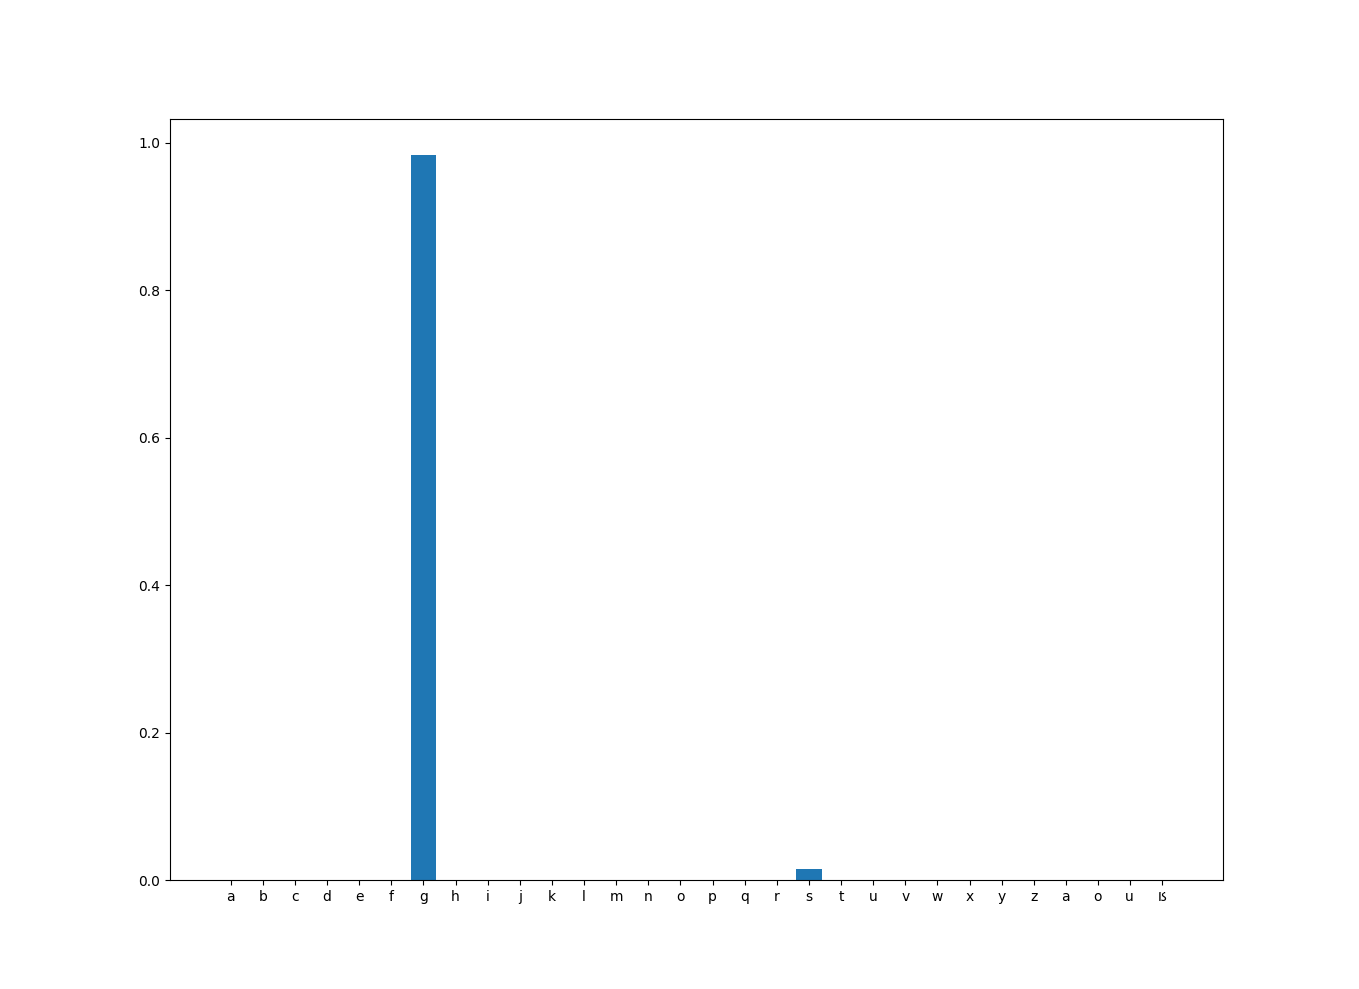
\includegraphics[width=\textwidth]{./plots/gunhistory.png}
	\item[c)]
	see prob\_dist.py\\
	\begin{table}[h]
		\begin{tabular}{l|c}
		 & Entropy \\ \hline
		 `'& 2.89886\\
		 `n'& 2.4599 \\
		 `un'& 1.22248\\
		 `gun'& 0.09247 \\
		\end{tabular}
	\end{table}
	We can see that the entropy grows to zero when the history grows, which is based on the fact that the probabilities are distributed on less characters with the minimum entropy 0 at one character with 100\%probability.
	\item[d)]
	Based on the observation in c) we know that the maximum entropy we be achieved if the probability would be evenly distributed among all characters, which would in the german alphabet result in the entropy:
	$$30* \frac{1}{30} * log(\frac{1}{30}) = log(\frac{1}{30}) = 1.47712125472  $$

	\item[e)]
	\begin{table}[h]
		\begin{tabular}{l|c}
		 & Entropy \\ \hline
		 `a'& 2.59749\\
		 `d'& 1.38149 \\
		 `z'& 1.86678\\
		 `c'& 0.55237 \\
		\end{tabular}
	\end{table}
	Below we have the plots for the histories `a', `d', `z' and `c'. This shows that not only the size of the historie is important for the probability distribution like we saw in part b). Even when the history has only one single character the distribution and with that the entropy can change a lot. The vocal a enables a lot of possible following characters based on the n-grams, which leads to a high entropy. d and z can lead to all the different letters in the alphabet but only 3 to 4 are realy frequent in the n-grams. This leads to a smaller entropy than for example the character a. The history c has a high probability to be followed by h, since `ch' is one combination often used in the german language. Since it is only one case with a realy high probability the entropy is quite small.

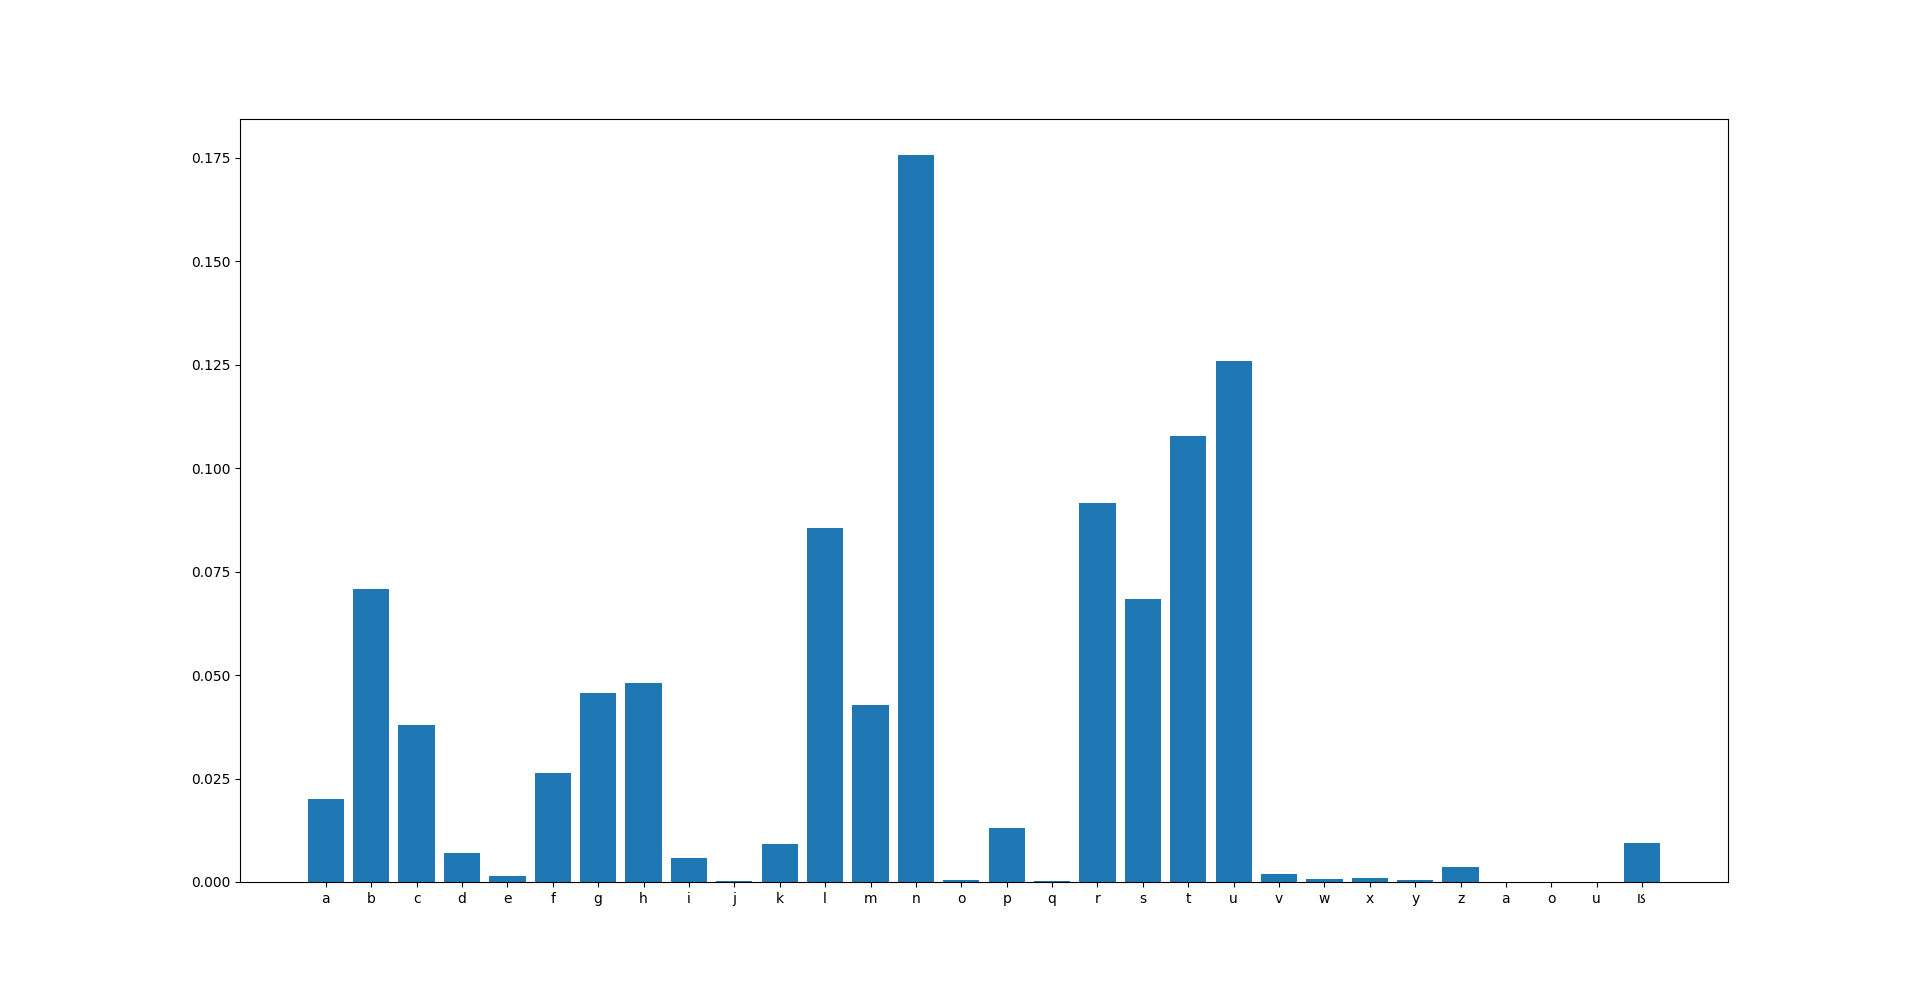
\includegraphics[width=\textwidth]{./plots/ahistory}
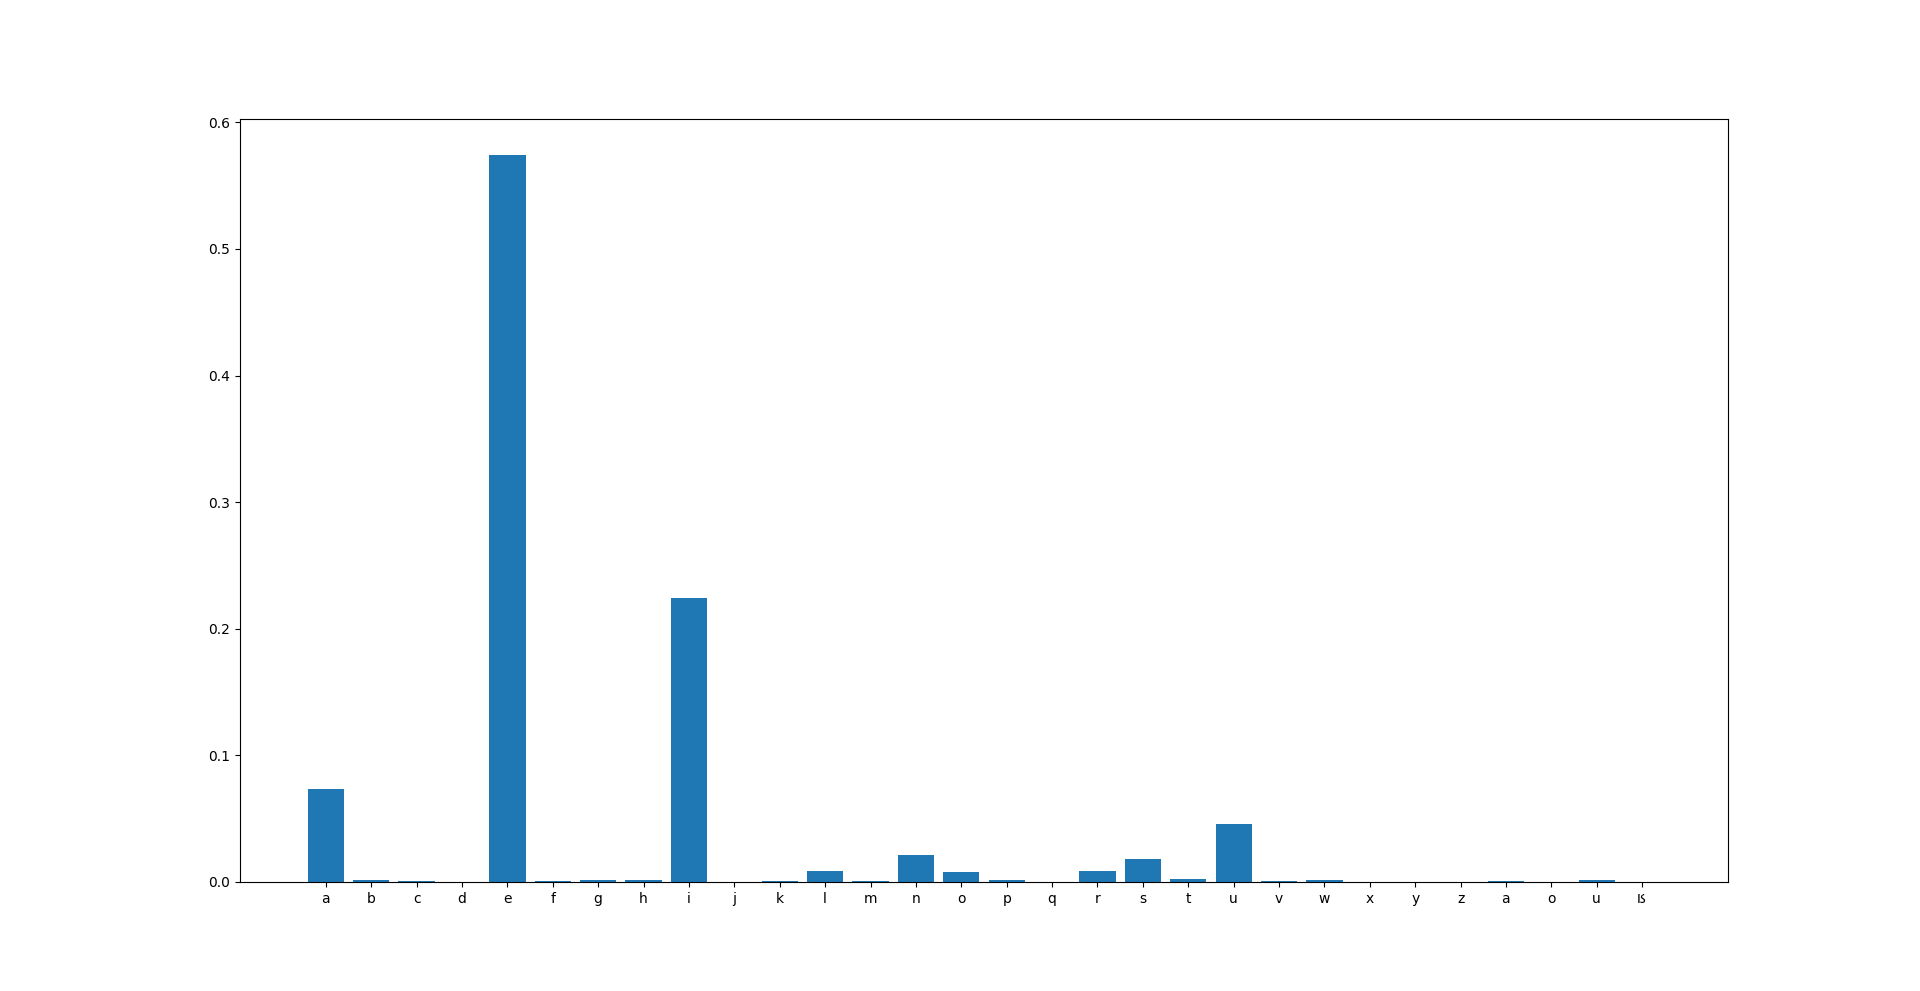
\includegraphics[width=\textwidth]{./plots/dhistory}
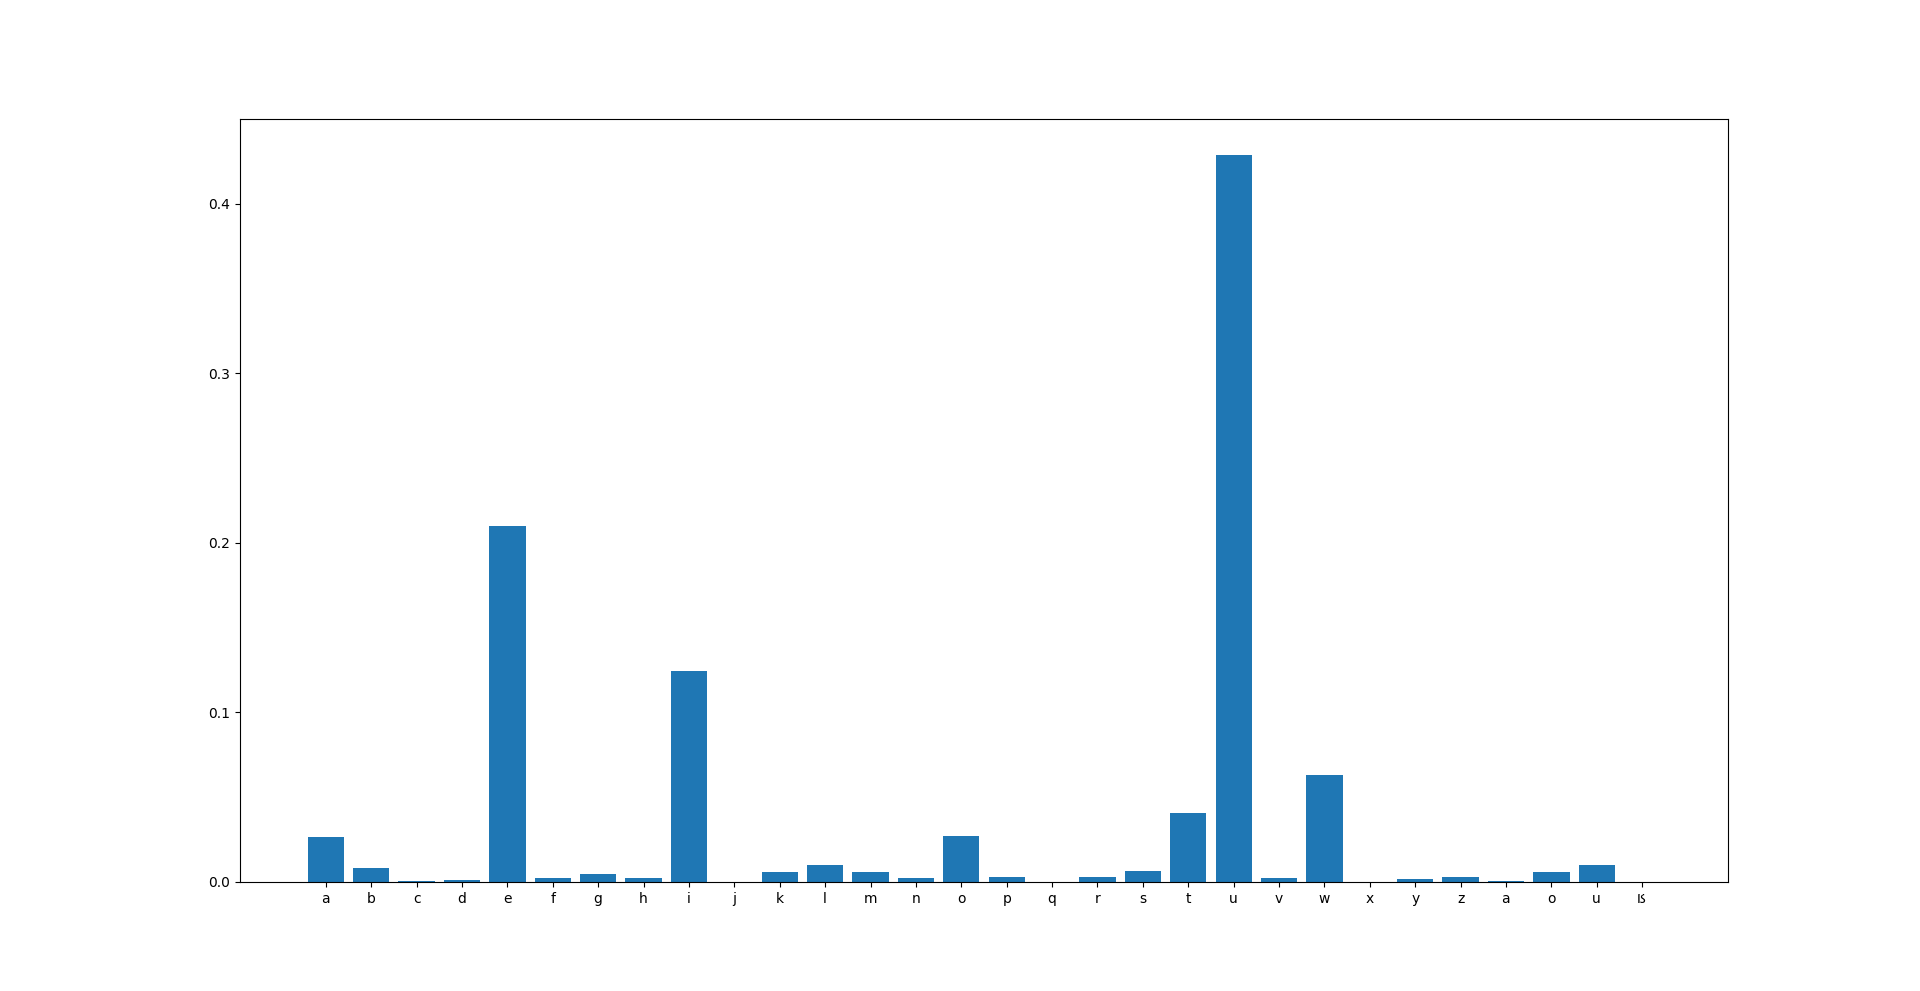
\includegraphics[width=\textwidth]{./plots/zhistory}
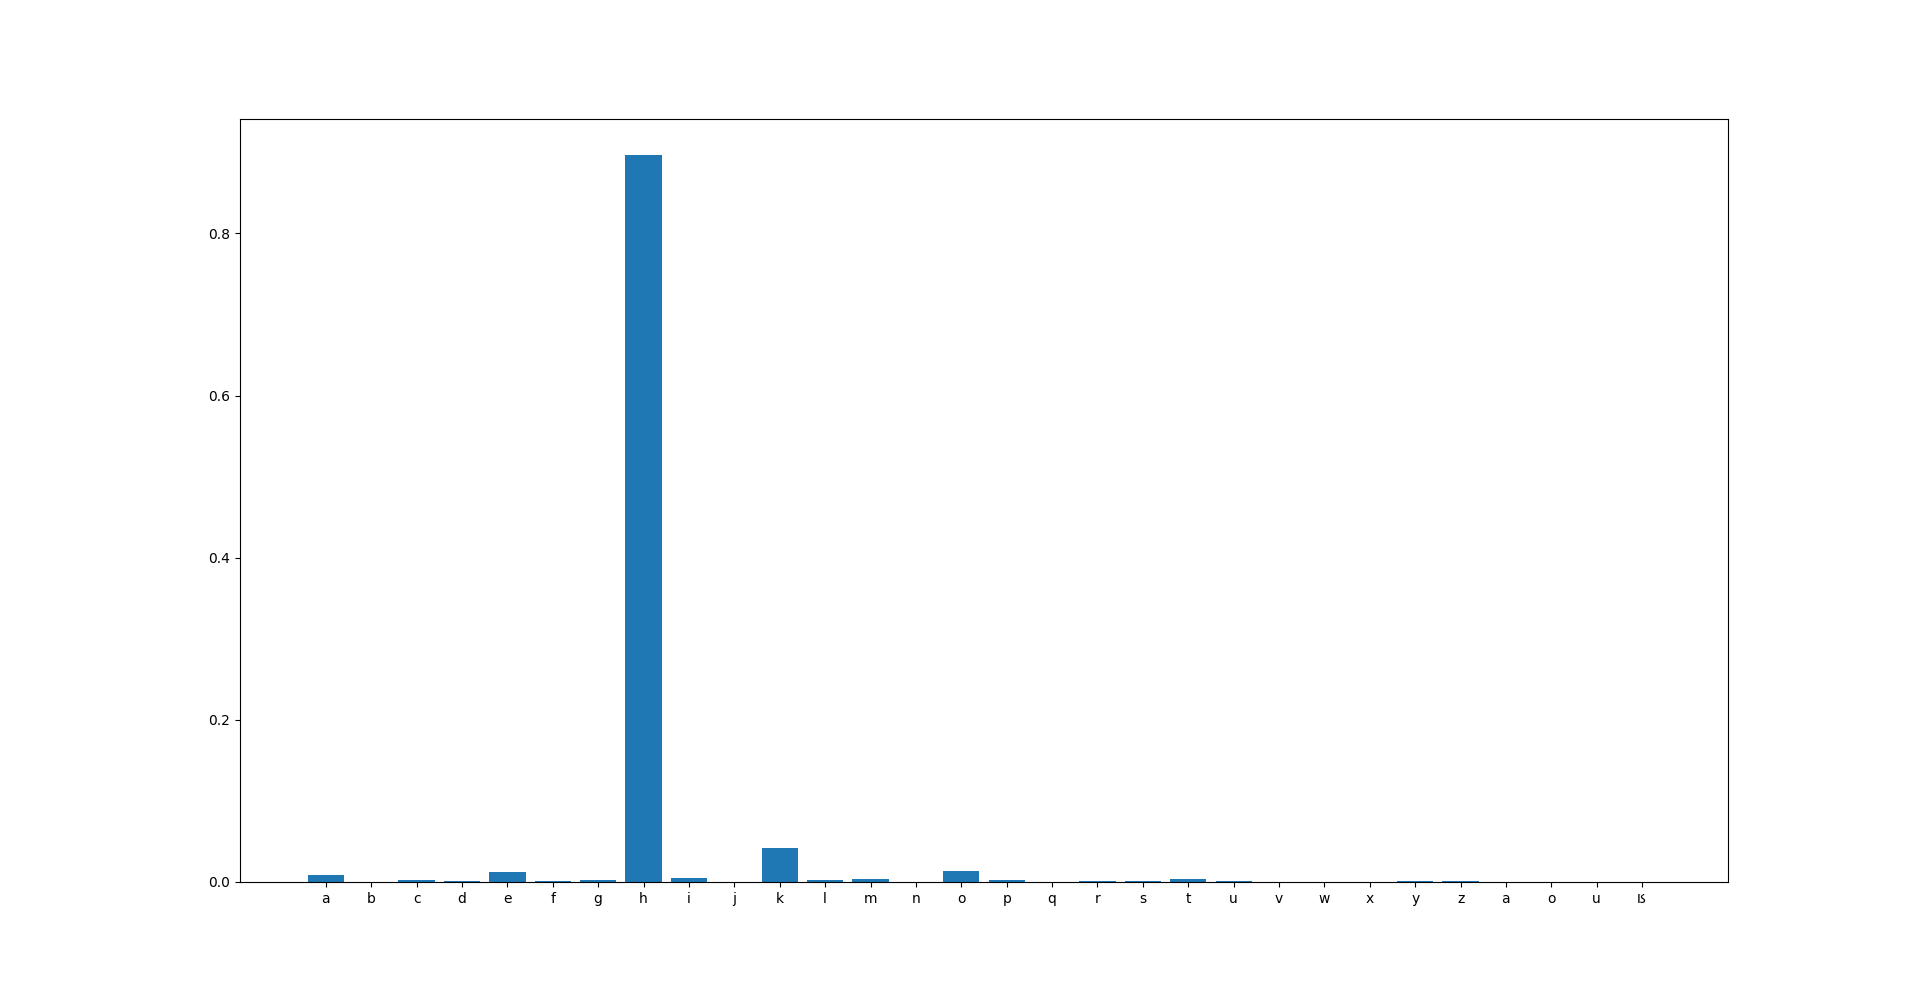
\includegraphics[width=\textwidth]{./plots/chistory}

\end{itemize}

\subsection{Cryptoanalysis}
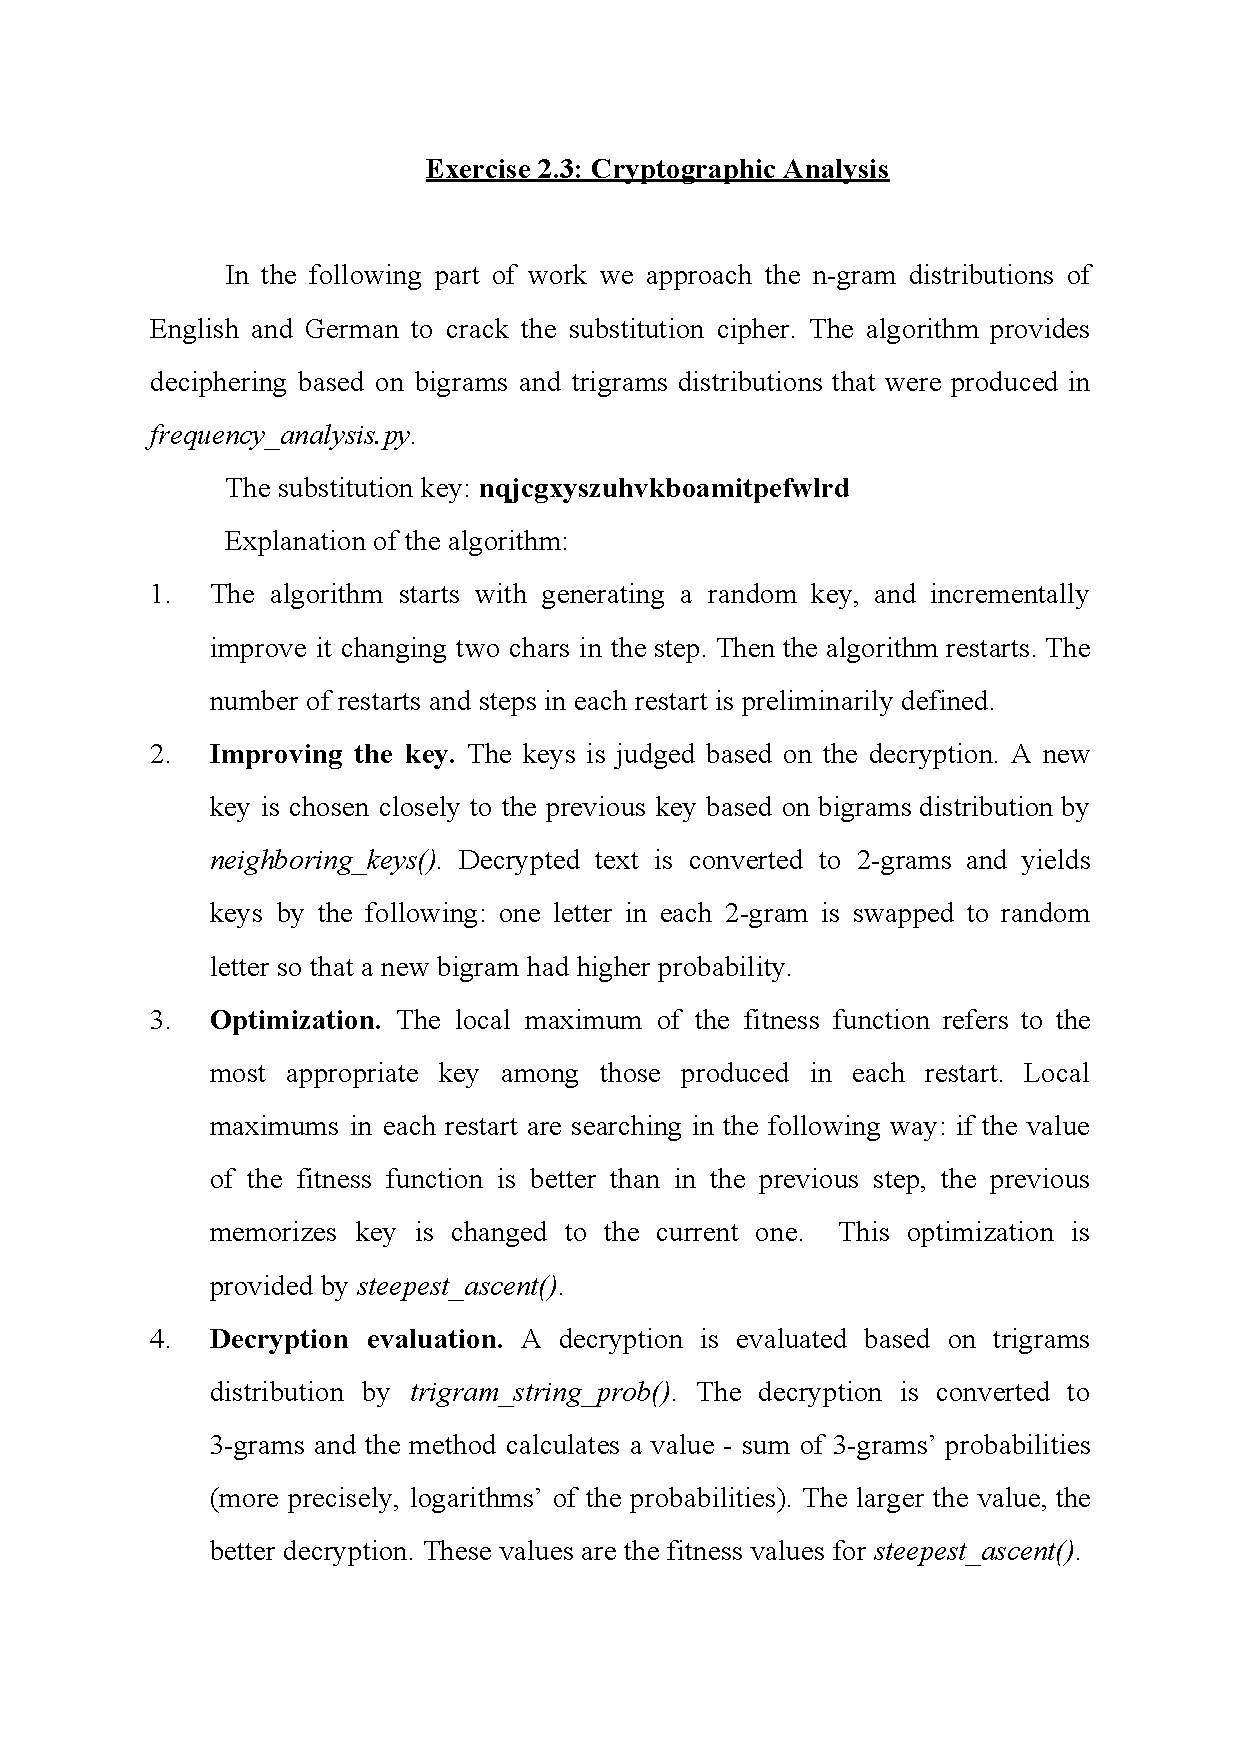
\includepdf[pages=-]{Ex23.pdf}

\end{document}
